% -*- coding: UTF-8 -*-
% vim: autoindent expandtab tabstop=4 sw=4 sts=4 filetype=tex
% vim: spelllang=de spell
% chktex-file 27 - disable warning about missing include files

\subsection{Vision}
\label{subsec:requirements:vision}

Der Autor dieser Projektarbeit stellt sich eine Software zur Verwaltung und
Darstellung von Echtzeit-Animationen vor. Die Software soll es Anwendern
erlauben Echtzeit-Animationen in intuitiver Weise zu erstellen. Sie soll zudem
modular gehalten sein, so dass spätere Änderungen, wie z.B.\ zusätzliche Arten
von Rendering, ohne Weiteres adaptierbar sind. Des Weiteren soll eine erstellte
Echtzeit-Animation mit geringem Aufwand exportiert werden können. Ein solcher
Export soll dann --- losgelöst vom Editor --- von einem Betrachter über eine
ausführbare Datei wiedergegeben werden können. Die Software besteht also
eigentlich aus zwei Applikationen: Dem \textit{Editor}, zum Erstellen und
Verwalten von Echtzeit-Animationen, sowie dem \textit{Player}, zum Betrachten
von Echtzeit-Animationen.

\autoref{fig:requirements:vision:editor-main} zeigt das mögliche Aussehen des
Editors und dessen Komponenten. Diese werden
in~\autoref{subsec:main-components:editor} erläutert.

\begin{figure}[H]
    \centering
    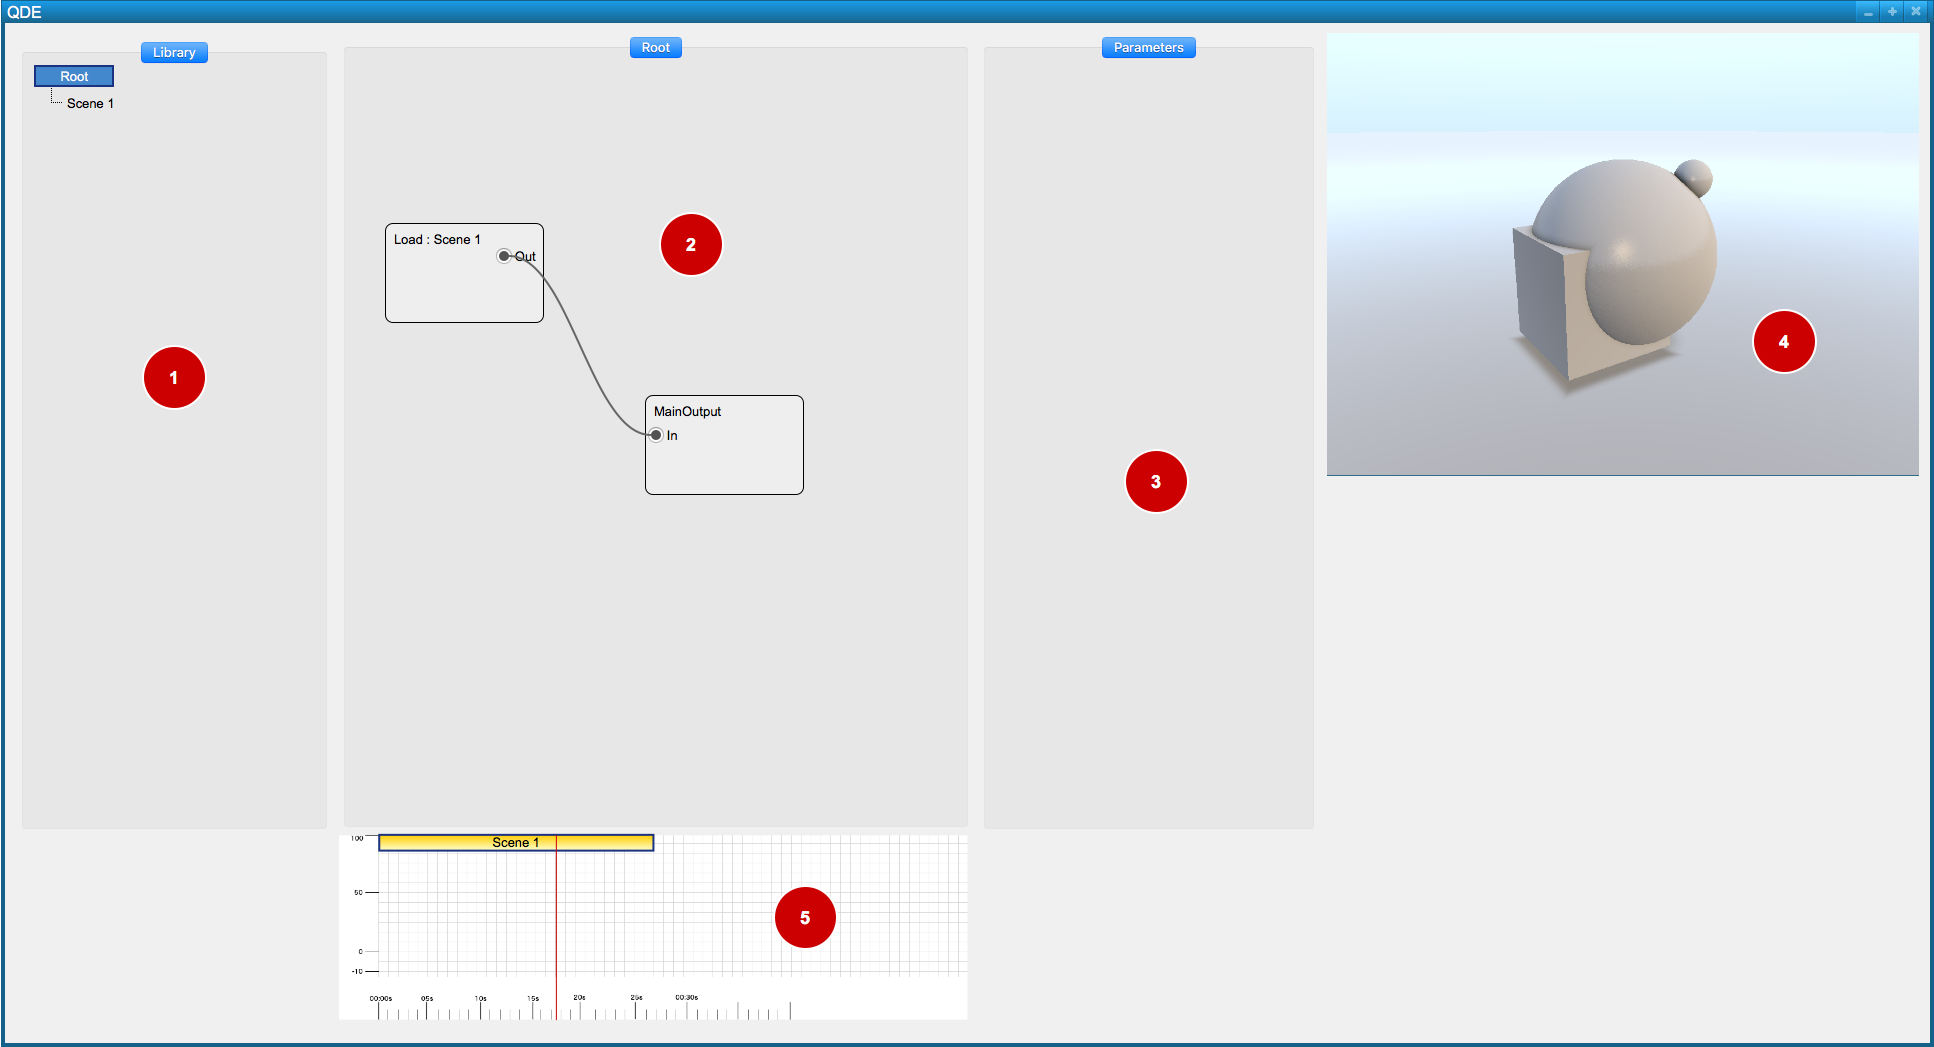
\includegraphics[width=0.9\textwidth]{img/editor_components.png}
    \caption{Mögliches Aussehen des Editors.}\label{fig:requirements:vision:editor-main}
\end{figure}
